\documentclass{standalone}
\usepackage{tikz}
\usetikzlibrary{patterns, positioning}
\usepackage[sfdefault]{ClearSans} %% option 'sfdefault' activates Clear Sans as the default text font
\usepackage[T1]{fontenc}

\begin{document}
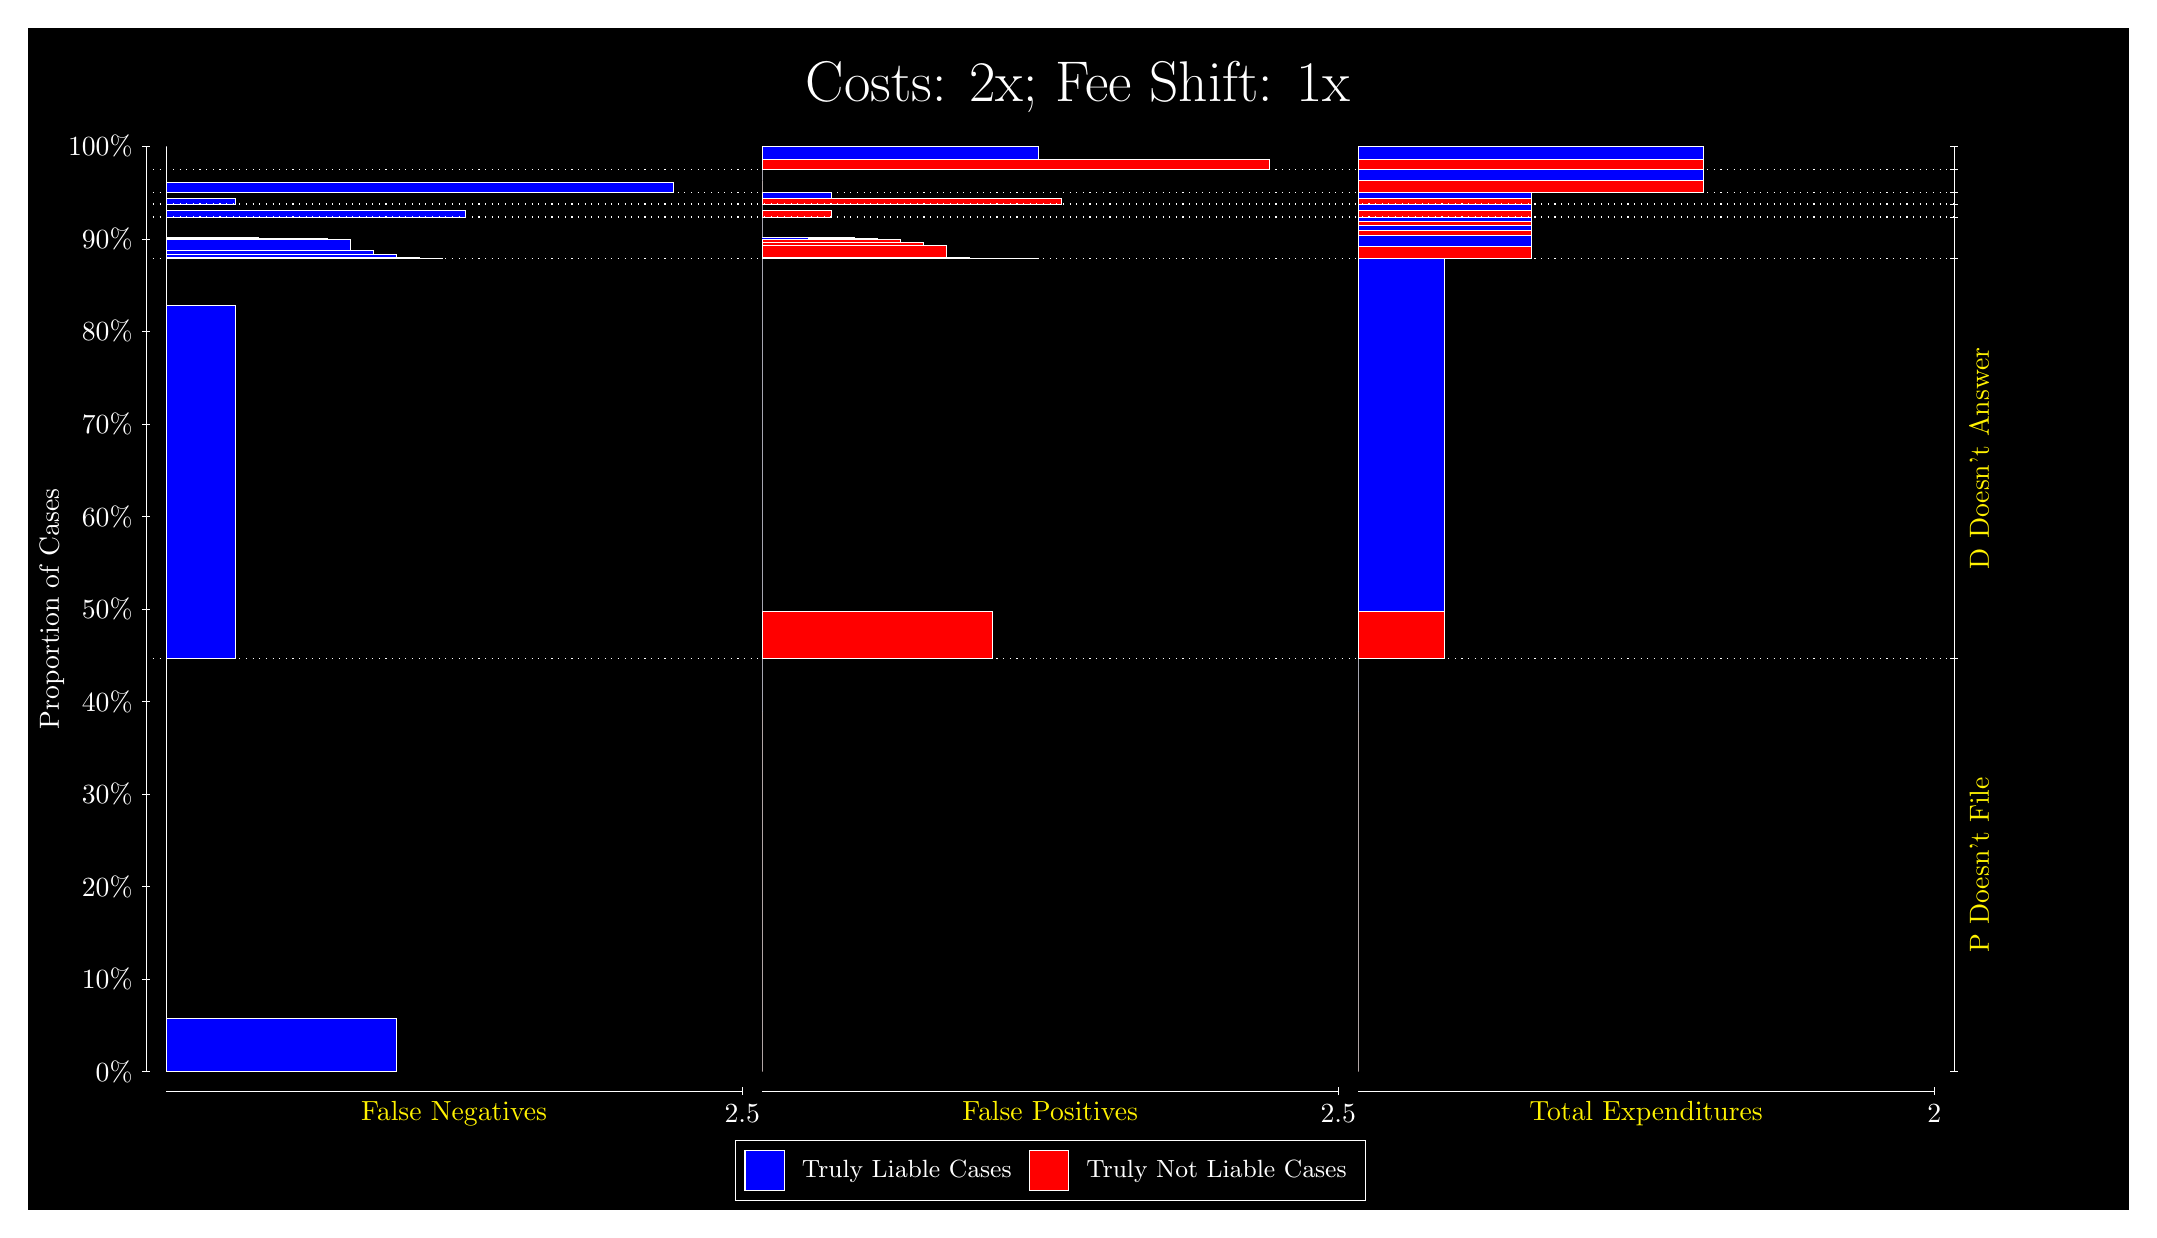
\begin{tikzpicture}
\draw[fill=black] (0,0) rectangle (26.667,15);
\draw[text=white] (0,13.5) rectangle (26.667,15) node[midway] {\huge Costs: 2x; Fee Shift: 1x};
\draw[white, very thin] (1.5,1.75) -- (1.5,13.5);
\node[rotate=90, text=white, anchor=center] at (0.3, 7.625) {Proportion of Cases};
\draw[white, very thin] (1.45,1.75) -- (1.55,1.75);
\node[text=white, anchor=east] at (1.45, 1.75) {0\%};
\draw[white, very thin] (1.45,2.925) -- (1.55,2.925);
\node[text=white, anchor=east] at (1.45, 2.925) {10\%};
\draw[white, very thin] (1.45,4.1) -- (1.55,4.1);
\node[text=white, anchor=east] at (1.45, 4.1) {20\%};
\draw[white, very thin] (1.45,5.275) -- (1.55,5.275);
\node[text=white, anchor=east] at (1.45, 5.275) {30\%};
\draw[white, very thin] (1.45,6.45) -- (1.55,6.45);
\node[text=white, anchor=east] at (1.45, 6.45) {40\%};
\draw[white, very thin] (1.45,7.625) -- (1.55,7.625);
\node[text=white, anchor=east] at (1.45, 7.625) {50\%};
\draw[white, very thin] (1.45,8.8) -- (1.55,8.8);
\node[text=white, anchor=east] at (1.45, 8.8) {60\%};
\draw[white, very thin] (1.45,9.975) -- (1.55,9.975);
\node[text=white, anchor=east] at (1.45, 9.975) {70\%};
\draw[white, very thin] (1.45,11.15) -- (1.55,11.15);
\node[text=white, anchor=east] at (1.45, 11.15) {80\%};
\draw[white, very thin] (1.45,12.325) -- (1.55,12.325);
\node[text=white, anchor=east] at (1.45, 12.325) {90\%};
\draw[white, very thin] (1.45,13.5) -- (1.55,13.5);
\node[text=white, anchor=east] at (1.45, 13.5) {100\%};

\draw[white, very thin] (24.457,1.75) -- (24.457,13.5);
\draw[white, very thin] (24.407,1.75) -- (24.507,1.75);
\node[anchor=west] at (24.407, 1.75) {};
\draw[white, very thin] (24.407,6.9958) -- (24.507,6.9958);
\node[anchor=west] at (24.407, 6.9958) {};
\draw[white, very thin] (24.407,12.076) -- (24.507,12.076);
\node[anchor=west] at (24.407, 12.076) {};
\draw[white, very thin] (24.407,12.603) -- (24.507,12.603);
\node[anchor=west] at (24.407, 12.603) {};
\draw[white, very thin] (24.407,12.768) -- (24.507,12.768);
\node[anchor=west] at (24.407, 12.768) {};
\draw[white, very thin] (24.407,12.913) -- (24.507,12.913);
\node[anchor=west] at (24.407, 12.913) {};
\draw[white, very thin] (24.407,13.204) -- (24.507,13.204);
\node[anchor=west] at (24.407, 13.204) {};
\draw[white, very thin] (24.407,13.5) -- (24.507,13.5);
\node[anchor=west] at (24.407, 13.5) {};

\draw[white, very thin, fill=blue] (1.75,1.75) rectangle (4.6775,2.4288);
\draw[white, very thin, fill=red] (1.75,2.4288) rectangle (1.75,6.9958);
\draw[white, very thin, fill=blue] (1.75,6.9958) rectangle (2.6283,11.479);
\draw[white, very thin, fill=red] (1.75,11.479) rectangle (1.75,12.076);
\draw[white, very thin, fill=blue] (1.75,12.076) rectangle (5.2631,12.084);
\draw[white, very thin, fill=blue] (1.75,12.084) rectangle (4.9703,12.093);
\draw[white, very thin, fill=blue] (1.75,12.093) rectangle (4.6775,12.134);
\draw[white, very thin, fill=blue] (1.75,12.134) rectangle (4.3848,12.135);
\draw[white, very thin, fill=blue] (1.75,12.135) rectangle (4.3848,12.178);
\draw[white, very thin, fill=blue] (1.75,12.178) rectangle (4.092,12.322);
\draw[white, very thin, fill=blue] (1.75,12.322) rectangle (3.7993,12.333);
\draw[white, very thin, fill=blue] (1.75,12.333) rectangle (3.5065,12.338);
\draw[white, very thin, fill=blue] (1.75,12.338) rectangle (3.2138,12.338);
\draw[white, very thin, fill=blue] (1.75,12.338) rectangle (2.921,12.339);
\draw[white, very thin, fill=red] (1.75,12.339) rectangle (1.75,12.603);
\draw[white, very thin, fill=blue] (1.75,12.603) rectangle (5.5558,12.682);
\draw[white, very thin, fill=red] (1.75,12.682) rectangle (1.75,12.768);
\draw[white, very thin, fill=blue] (1.75,12.768) rectangle (2.6283,12.844);
\draw[white, very thin, fill=red] (1.75,12.844) rectangle (1.75,12.913);
\draw[white, very thin, fill=blue] (1.75,12.913) rectangle (8.1906,13.049);
\draw[white, very thin, fill=red] (1.75,13.049) rectangle (1.75,13.204);
\draw[white, very thin, fill=red] (1.75,13.204) rectangle (1.75,13.341);
\draw[white, very thin, fill=blue] (1.75,13.341) rectangle (1.75,13.5);
\draw[white, very thin, fill=red] (9.3189,1.75) rectangle (9.3189,6.317);
\draw[white, very thin, fill=blue] (9.3189,6.317) rectangle (9.3189,6.9958);
\draw[white, very thin, fill=red] (9.3189,6.9958) rectangle (12.246,7.5927);
\draw[white, very thin, fill=blue] (9.3189,7.5927) rectangle (9.3189,12.076);
\draw[white, very thin, fill=red] (9.3189,12.076) rectangle (12.832,12.077);
\draw[white, very thin, fill=red] (9.3189,12.077) rectangle (12.539,12.078);
\draw[white, very thin, fill=red] (9.3189,12.078) rectangle (12.246,12.082);
\draw[white, very thin, fill=red] (9.3189,12.082) rectangle (11.954,12.094);
\draw[white, very thin, fill=red] (9.3189,12.094) rectangle (11.661,12.238);
\draw[white, very thin, fill=red] (9.3189,12.238) rectangle (11.368,12.281);
\draw[white, very thin, fill=red] (9.3189,12.281) rectangle (11.075,12.323);
\draw[white, very thin, fill=red] (9.3189,12.323) rectangle (10.783,12.332);
\draw[white, very thin, fill=red] (9.3189,12.332) rectangle (10.49,12.34);
\draw[white, very thin, fill=blue] (9.3189,12.34) rectangle (9.9044,12.341);
\draw[white, very thin, fill=blue] (9.3189,12.341) rectangle (9.6116,12.342);
\draw[white, very thin, fill=blue] (9.3189,12.342) rectangle (9.3189,12.603);
\draw[white, very thin, fill=red] (9.3189,12.603) rectangle (10.197,12.689);
\draw[white, very thin, fill=blue] (9.3189,12.689) rectangle (9.3189,12.768);
\draw[white, very thin, fill=red] (9.3189,12.768) rectangle (13.125,12.837);
\draw[white, very thin, fill=blue] (9.3189,12.837) rectangle (10.197,12.913);
\draw[white, very thin, fill=red] (9.3189,12.913) rectangle (9.3189,13.068);
\draw[white, very thin, fill=blue] (9.3189,13.068) rectangle (9.3189,13.204);
\draw[white, very thin, fill=red] (9.3189,13.204) rectangle (15.759,13.341);
\draw[white, very thin, fill=blue] (9.3189,13.341) rectangle (12.832,13.5);
\draw[white, very thin, fill=red] (16.888,1.75) rectangle (16.888,6.317);
\draw[white, very thin, fill=blue] (16.888,6.317) rectangle (16.888,6.9958);
\draw[white, very thin, fill=red] (16.888,6.9958) rectangle (17.986,7.5927);
\draw[white, very thin, fill=blue] (16.888,7.5927) rectangle (17.986,12.076);
\draw[white, very thin, fill=red] (16.888,12.076) rectangle (19.083,12.226);
\draw[white, very thin, fill=blue] (16.888,12.226) rectangle (19.083,12.375);
\draw[white, very thin, fill=red] (16.888,12.375) rectangle (19.083,12.435);
\draw[white, very thin, fill=blue] (16.888,12.435) rectangle (19.083,12.494);
\draw[white, very thin, fill=red] (16.888,12.494) rectangle (19.083,12.549);
\draw[white, very thin, fill=blue] (16.888,12.549) rectangle (19.083,12.603);
\draw[white, very thin, fill=red] (16.888,12.603) rectangle (19.083,12.689);
\draw[white, very thin, fill=blue] (16.888,12.689) rectangle (19.083,12.768);
\draw[white, very thin, fill=red] (16.888,12.768) rectangle (19.083,12.837);
\draw[white, very thin, fill=blue] (16.888,12.837) rectangle (19.083,12.913);
\draw[white, very thin, fill=red] (16.888,12.913) rectangle (21.279,13.068);
\draw[white, very thin, fill=blue] (16.888,13.068) rectangle (21.279,13.204);
\draw[white, very thin, fill=red] (16.888,13.204) rectangle (21.279,13.341);
\draw[white, very thin, fill=blue] (16.888,13.341) rectangle (21.279,13.5);
\draw[white, dotted] (1.5,6.9958) -- (24.457,6.9958);
\draw[white, dotted] (1.5,12.076) -- (24.457,12.076);
\draw[white, dotted] (1.5,12.603) -- (24.457,12.603);
\draw[white, dotted] (1.5,12.768) -- (24.457,12.768);
\draw[white, dotted] (1.5,12.913) -- (24.457,12.913);
\draw[white, dotted] (1.5,13.204) -- (24.457,13.204);
\draw[white, very thin] (1.75,1.5) -- (9.0689,1.5);
\node[text=yellow, anchor=north] at (5.4094, 1.5) {False Negatives};
\draw[white, very thin] (9.0689,1.45) -- (9.0689,1.55);
\node[text=white, anchor=north] at (9.0689, 1.45) {2.5};

\draw[white, very thin] (9.3189,1.5) -- (16.638,1.5);
\node[text=yellow, anchor=north] at (12.978, 1.5) {False Positives};
\draw[white, very thin] (16.638,1.45) -- (16.638,1.55);
\node[text=white, anchor=north] at (16.638, 1.45) {2.5};

\draw[white, very thin] (16.888,1.5) -- (24.207,1.5);
\node[text=yellow, anchor=north] at (20.547, 1.5) {Total Expenditures};
\draw[white, very thin] (24.207,1.45) -- (24.207,1.55);
\node[text=white, anchor=north] at (24.207, 1.45) {2};

\node[text=yellow, centered, rotate=90] at (24.777, 4.3729) {P Doesn't File};
\node[text=yellow, centered, rotate=90] at (24.777, 9.5361) {D Doesn't Answer};






\draw (12.978300999999998,1.5) node[draw=none] (baseCoordinate) {};
\begin{scope}[align=center]
        \matrix[scale=0.5, draw=white, below=0.5cm of baseCoordinate, nodes={draw}, column sep=0.1cm]{
            \node[rectangle, draw, minimum width=0.5cm, minimum height=0.5cm, fill=blue] {}; &
            \node[draw=none, font=\small, text=white] (B) {Truly Liable Cases}; &
            \node[rectangle, draw, minimum width=0.5cm, minimum height=0.5cm, fill=red] {}; &
            \node[draw=none, font=\small, text=white] (B) {Truly Not Liable Cases}; \\
            };
\end{scope}

\end{tikzpicture}
\end{document}